\appendix

\begin{figure}[h]
  \centering
  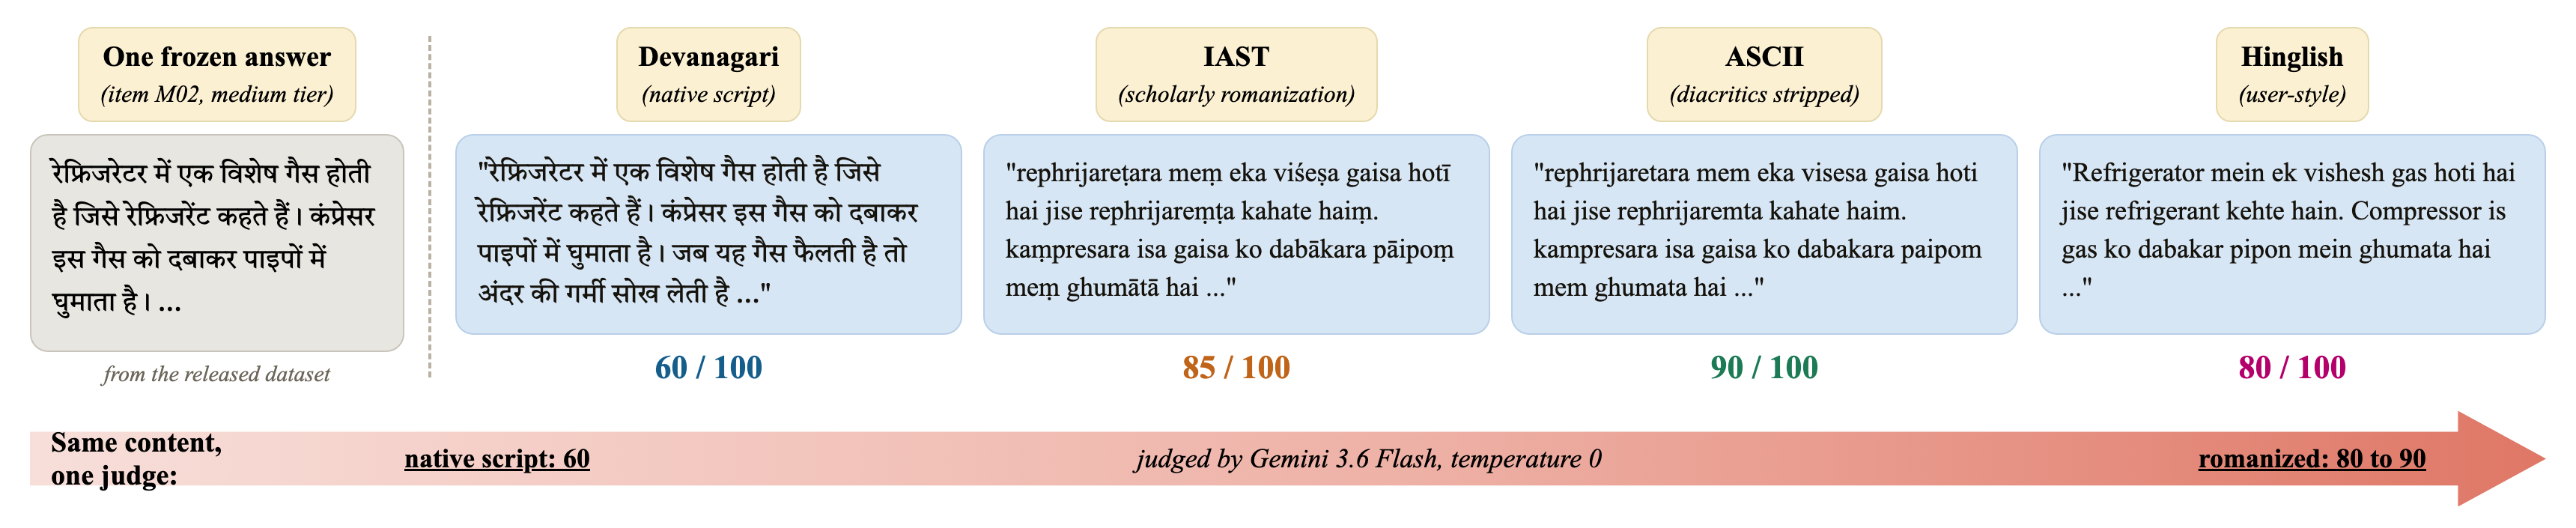
\includegraphics[width=0.75\textwidth]{assets/fig6_example.png}
  \caption{\textbf{Qualitative example (item M02).} Same content, four orthographies, one judge: scores of 60 (Devanagari), 85, 90, and 80 (romanized), verbatim from the released data.}
  \label{fig:example}
\end{figure}


\section{Verbatim judging prompts}
\label{app:prompts}

\textbf{Main rubric} (all core arms; \texttt{\{instruction\}} and \texttt{\{response\}} substituted per item):
\begin{quote}\small\ttfamily
You are grading one response to one instruction for an instruction-following benchmark.\\
Score the response from 0 to 100 considering: correctness (facts right), completeness (covers what the instruction asks), helpfulness, and clarity.\\
Judge this item on its own merits.\\
Instruction: \{instruction\}\\
Response: \{response\}\\
Reply with ONLY a JSON object: \{"score": <integer 0-100>, "reason": "<one short sentence>"\}
\end{quote}

\textbf{Decomposed rubric} (sub-dimension battery and mitigation arm R1):
\begin{quote}\small\ttfamily
Give four sub-scores from 0 to 25 each: correctness (facts right), completeness (covers what the instruction asks), helpfulness, clarity. The total is their sum. [...] Reply with ONLY a JSON object: \{"correctness": <0-25>, "completeness": <0-25>, "helpfulness": <0-25>, "clarity": <0-25>, "score": <integer 0-100 sum>, "reason": "..."\}
\end{quote}

\textbf{Pairwise prompt} (deva-versus-ascii battery; A/B assignment counterbalanced):
\begin{quote}\small\ttfamily
You are comparing two responses to the same instruction for an instruction-following benchmark. Decide which response is better overall considering correctness, completeness, helpfulness, and clarity. If they are equally good, say tie. [...] Reply with ONLY a JSON object: \{"winner": "A" or "B" or "tie", "reason": "..."\}
\end{quote}

\textbf{Batched protocol control}: the main rubric's scoring instruction, followed by 25 numbered instruction-response items and a request for a JSON array of \{n, score, reason\} objects, submitted through the same headless interface as the one-per-call arm.

The five mitigation-arm phrasings (P1-P5) are given in \S\ref{sec:mitigation}; all prompts also ship verbatim in the released run scripts.

\section{Follow-up battery tables}
\label{app:followup}

All values are mean within-item paired differences versus the Devanagari twin, with bootstrap 95\% CIs (10{,}000 resamples) and two-sided sign-flip permutation $p$ (20{,}000 permutations), from the released \texttt{analysis\_batteries.json}.

\begin{table}[h]
\centering\small
\caption{GPT-5.6 core battery (one item per call, temperature 0, unified OpenAI-compatible gateway), $n{=}150$ per condition (149 for ASCII; one unparsed call).}
\begin{tabular}{lcccc}
\toprule
Condition & Shift & 95\% CI & $p$ & by tier (high/med/low) \\
\midrule
IAST & $+1.21$ & $[+0.18, +2.23]$ & $0.023$ & $+0.40$ / $-0.60$ / $+3.84$ \\
ASCII & $+0.51$ & $[-0.61, +1.66]$ & $0.384$ & $-1.84$ / $+0.26$ / $+3.06$ \\
Hinglish & $+0.62$ & $[-0.23, +1.48]$ & $0.157$ & $+0.02$ / $+0.56$ / $+1.28$ \\
\bottomrule
\end{tabular}
\end{table}

\begin{table}[h]
\centering\small
\caption{Per-dimension decomposition of the ASCII-versus-Devanagari shift (0-25 scale per dimension), $n{=}150$ pairs per judge. Sonnet 5 via the headless one-per-call interface; Flash via its native API at temperature 0.}
\begin{tabular}{lcccc}
\toprule
Judge & Correctness & Completeness & Helpfulness & Clarity \\
\midrule
Claude Sonnet 5 & $-1.57$ {\scriptsize$p{=}5{\times}10^{-5}$} & $-0.21$ {\scriptsize$p{=}0.18$} & $-0.54$ {\scriptsize$p{=}0.001$} & $-4.82$ {\scriptsize$p{=}5{\times}10^{-5}$} \\
Gemini 3.6 Flash & $-0.39$ & $+0.37$ & $+0.22$ & $-2.29$ \\
\bottomrule
\end{tabular}
\end{table}

\begin{table}[h]
\centering\small
\caption{Pairwise deva-versus-ascii preference, both presentation orders, 300 trials per judge.}
\begin{tabular}{lccccc}
\toprule
Judge & Deva wins & ASCII wins & Ties & Sign-test $p$ & Deva-first / ASCII-first splits \\
\midrule
Gemini 3.6 Flash & 288 & 0 & 12 & $4.0\times10^{-87}$ & 149-0-1 / 139-0-11 \\
Claude Sonnet 5 & 293 & 0 & 7 & $1.3\times10^{-88}$ & — \\
\bottomrule
\end{tabular}
\end{table}

\begin{table}[h]
\centering\small
\caption{Protocol control, Claude Sonnet 5: identical items, identical headless interface and per-item rubric; only batch size differs. $n{=}150$ per cell.}
\begin{tabular}{lcccc}
\toprule
Protocol & IAST & ASCII & Hinglish & ASCII by tier (h/m/l) \\
\midrule
One per call & $-2.70$ & $-12.29$ & $-2.71$ & $-24.28$ / $-12.96$ / $+0.38$ \\
Batched (25/call) & $+2.64$ & $+1.12$ & $-1.29$ & $-3.62$ / $+3.48$ / $+3.50$ \\
\bottomrule
\end{tabular}
\end{table}

\textbf{Test-retest.} 30 stratified items, deva and ascii, five identical Flash calls each at temperature 0: mean within-item SD $1.66$, mean range $3.33$, 28 of 60 item-conditions perfectly stable across all five calls.

\textbf{FDR correction.} Benjamini-Hochberg over all 198 reported p-values: 108 remain significant at $q{=}0.05$, including every effect named in the abstract. The full per-test table ships in \texttt{analysis\_extra.json}.

\textbf{Logit-scale tier reanalysis} (Flash). Transforming scores by $\mathrm{logit}(s/100)$ (clipped to $[0.5, 99.5]$) before differencing removes bounded-scale compression. The medium tier retains the largest shift under all three romanizations (logit shifts $+0.29$ to $+0.35$, versus at most $+0.22$ for high and low tiers, and $-0.48$ for high-tier ASCII), so the discretion account survives the transform.

\textbf{Qwen leading-token distribution.} Top-20 logprobs at the first score token (leading digit for two-digit scores): expectation $5.70$ (deva), $6.33$ (IAST), $6.17$ (ASCII), $5.73$ (Hinglish); within-call SD $0.60$ to $0.62$ throughout, consistent with a mode move rather than a widening.
